\documentclass{article}

% Bibliography
\usepackage{natbib}
\bibpunct{(}{)}{;}{a}{}{;}

% Use 'It was found that A is B (Name 1234)' style
\setcitestyle{authoryear,open={},close={}}

% Affiliations
\usepackage{authblk}
\title{pirouette: the error BEAST2 makes in inferring a phylogeny}
\author[1]{Rich\`el J.C. Bilderbeek}
\author[1]{Giovanni Laudanno}
\author[1]{Rampal S. Etienne}
\affil[1]{Groningen Institute for Evolutionary Life Sciences, University of Groningen, Groningen, The Netherlands}

% Use double spacing
\usepackage{setspace}
\doublespacing

\usepackage{listings}
\usepackage{hyperref}
\usepackage{todonotes}
\usepackage{verbatim}
\usepackage{pgf}
\usepackage{bm}

% sidewaysfigure
\usepackage{rotating}

% Style of listings
% From http://r.789695.n4.nabble.com/How-to-nicely-display-R-code-with-the-LaTeX-package-listings-tp4648110.html
\usepackage{fancyvrb} 
\definecolor{codegreen}{rgb}{0,0.6,0}
\definecolor{codegray}{rgb}{0.5,0.5,0.5}
\definecolor{codepurple}{rgb}{0.58,0,0.82}
\definecolor{backcolor}{rgb}{0.95,0.95,0.92}
\lstdefinestyle{mystyle}{
  language=R,% set programming language
  basicstyle=\ttfamily\small,% basic font style
  commentstyle=\color{gray},% comment style
  % numbers=left,% display line numbers on the left side
  numberstyle=\scriptsize,% use small line numbers
  numbersep=10pt,% space between line numbers and code
  tabsize=2,% sizes of tabs
  showstringspaces=false,% do not replace spaces in strings by a certain character
  captionpos=b,% positioning of the caption below
  breaklines=true,% automatic line breaking
  escapeinside={(*}{*)},% escaping to LaTeX
  fancyvrb=true,% verbatim code is typset by listings
  extendedchars=false,% prohibit extended chars (chars of codes 128--255)
  alsoletter={.<-},% becomes a letter
  alsoother={$},% becomes other
  otherkeywords={!=, ~, $, \&, \%/\%, \%*\%, \%\%, <-, <<-, /},% other keywords
  deletekeywords={c}% remove keywords 
}
\lstset{style=mystyle}

% Adds numbered lines
\usepackage{lineno}
\linenumbers

% Rename 'Abstract' to 'Summary 
\usepackage[english]{babel}
\addto{\captionsenglish}{\renewcommand{\abstractname}{Summary}}

\begin{document}

\maketitle

\begin{abstract}

  \textbf{1. }
    BEAST2 is a popular Bayesian phylogenetics software tool,
    that takes an alignment and inference model to create a
    posterior of jointly-estimated phylogenies and model parameter estimates.
    When a new macro-evolutionary speciation model is developed,
    a good first step is to measure the error BEAST2 makes on known
    phylogeny derived from the new speciation process, 
    with its current set of inference models. \\
  \textbf{2. }
    Here, we present a free, libre and open-source R package, \verb;pirouette;
    that assesses the inference error BEAST2 makes based on a known/true 
    phylogeny. \\
  \textbf{3. }
    We describe \verb;pirouette;'s usage and the biological scientific
    question it can answer, including full examples. \\
  \textbf{4. }
    As \verb;pirouette; is designed to be of high quality and extendable, 
    we conclude by describing the further development of the package. \\
\end{abstract}

{\bf Keywords:} computational biology, evolution, phylogenetics, BEAST2, pirouette, R





%%%%%%%%%%%%%%%%%%%%%%%%%%%%%%%%%%%%%%%%%%%%%%%%%%%%%%%%%%%%%%%%%%%%%%%%%%%%%%%%%%%%%%
\section{Introduction}
%%%%%%%%%%%%%%%%%%%%%%%%%%%%%%%%%%%%%%%%%%%%%%%%%%%%%%%%%%%%%%%%%%%%%%%%%%%%%%%%%%%%%%

Phylogenies are commonly used to explore evolutionary hypotheses.

%%%%%%%%%%%%%%%%%%%%%%%%%%%%%%%%%%%%%%%%%%%%%%%%%%%%%%%%%%%%%%%%%%%%%%%%%%%%%%%%%%%%%%
\section{Description}
%%%%%%%%%%%%%%%%%%%%%%%%%%%%%%%%%%%%%%%%%%%%%%%%%%%%%%%%%%%%%%%%%%%%%%%%%%%%%%%%%%%%%%

\verb;pirouette; is written in the R programming language (\cite{R}).

\begin{sidewaysfigure}
  \centering
  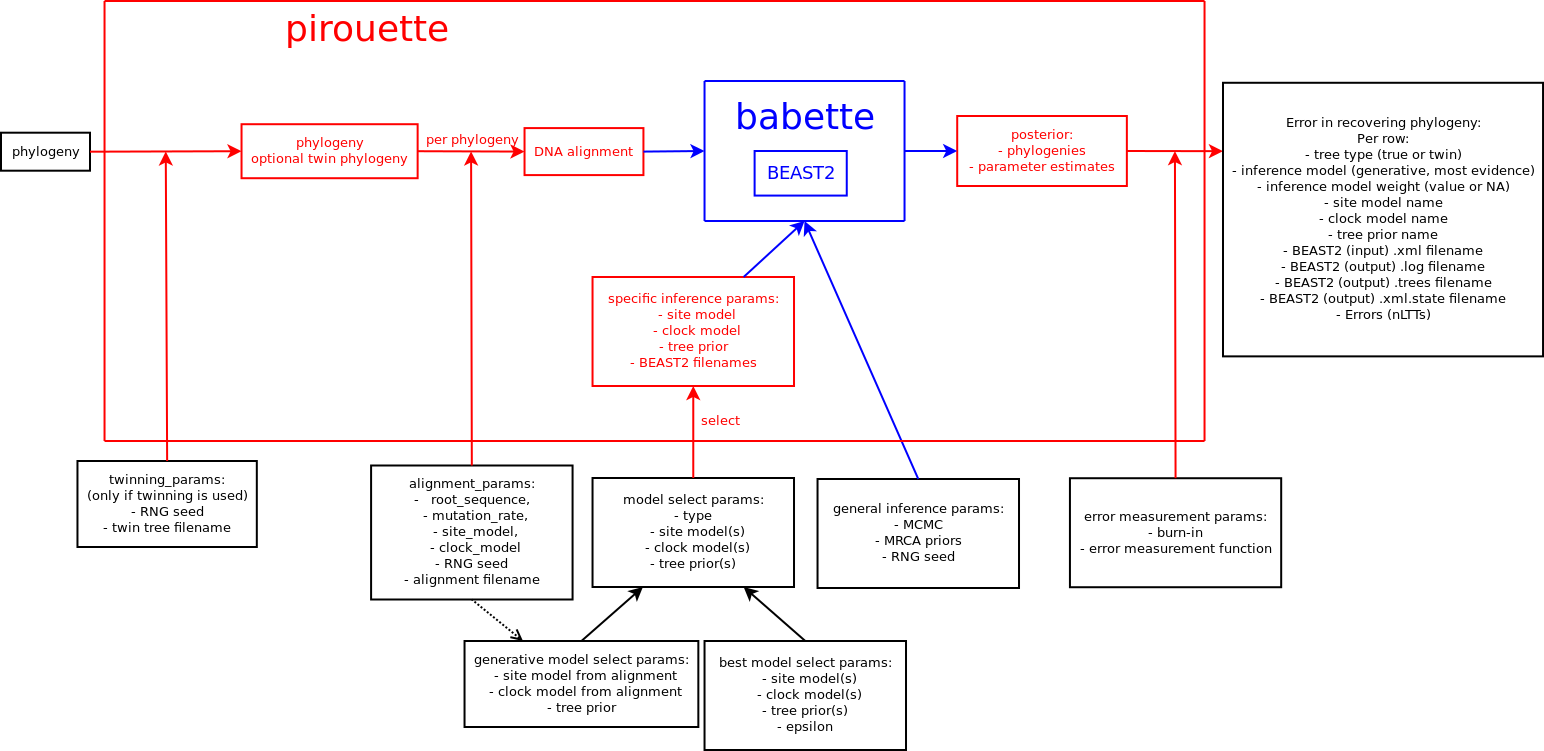
\includegraphics[width=\textwidth]{overview.png}
  \caption{pirouette pipeline}
  \label{fig:pipeline}
\end{sidewaysfigure}

The goal of \verb;pirouette; is to measure the inference error BEAST2
makes from a given/known/true phylogeny. This involves multiple steps,
described in detail below. 
In brief: from a given phylogeny, an alignment is simulated, from which a BEAST2
posterior is inferred, of which its phylogenies are compared with the given
phylogeny. The more the posterior phylogenies match the given phylogeny,
the lower the error. The is also the option to generate a 'twin tree',
that goes through the same pipeline.

The first step simulates a DNA alignment from the given phylogeny.
One can specify a DNA sequence
of any length at the root of the phylogeny, a DNA mutation rate, a
site (also: nucleotide substitution) model, 
a clock model, a random number generator (RNG) seed and a location
where the alignment is saved to. This step is relatively fast, but longer
DNA alignments will noticably slow down the inference step.

The second step selects an inference model, using the alignment.
The user can specify to use the generative model or select a best model
from a set of inference models. 
When selecting the generative model,
the site and clock model used in the alignment simulation are used
in inference. Because the given phylogeny (on which the alignment is based)
may have followed any tree prior (also: speciation model), the user needs
to specify which tree prior is used in inference. 
When selecting a best
model, the alignment is used to find the inference model that has the
highest evidence (also: marginal likelihood) from a set of inference models.
The evidence of an inference model is estimated using a nested-sampling
approach, as decribed in Maturana et al., 2018. The nested sampling is
performed by \verb;babette;, that call the 'NS' BEAST2 package. 
Using BEAST2 packages (in a scripted way) can only be done under Linux and Mac,
which excludes Windows from this way of selecting an inference model.

The third step infers a Bayesian posterior from the simulated alignment,
using the inference model(s) selected in the previous step. The user
can specify the additional parameters needed for a BEAST2 run, which
are the Markov-Chain Monte Carlo (MCMC) setup, 
an optional Most Recent Common Ancestor (MRCA) prior and an RNG seed.
The MCMC setup determines the number of posterior trees sampled.
An MRCA prior allows the inferred phylogeny to have a dated crown age.

The fourth step measures the inference error, using the phylogenies in the
Bayesian posterior. These phylogenies are compared to the given
phylogeny using an error statistic, which is the nLTT 
statistic [Janzen et al., ?2016]. Additionally, the user can specify the
propertion of posterior phylogenies to discard (also called: the burn-in).

An optional step is to generate a 'twin tree', that will be
analyzed in the same way as the true tree.

%%%%%%%%%%%%%%%%%%%%%%%%%%%%%%%%%%%%%%%%%%%%%%%%%%%%%%%%%%%%%%%%%%%%%%%%%%%%%%%%%%%%%%
\section{Installation}
%%%%%%%%%%%%%%%%%%%%%%%%%%%%%%%%%%%%%%%%%%%%%%%%%%%%%%%%%%%%%%%%%%%%%%%%%%%%%%%%%%%%%%

\verb;pirouette; can be installed easily from CRAN:

\begin{lstlisting}[language=R, floatplacement=H]
install.packages("piouette")
\end{lstlisting}

For the most up-to-date version, 
one can download and install the package from \verb;pirouette;'s GitHub repository:

\begin{lstlisting}[language=R, floatplacement=H]
usthis::install_github("richelbilderbeek/pirouette")
\end{lstlisting}
To start using \verb;pirouette;, load its functions in the global namespace first:

\begin{lstlisting}[language=R, floatplacement=H]
library(pirouette)
\end{lstlisting}
Because \verb;pirouette; calls BEAST2, BEAST2 must be installed. 
This can be done from within R, using:

\begin{lstlisting}[language=R, floatplacement=H]
install_beast2()
\end{lstlisting}


%%%%%%%%%%%%%%%%%%%%%%%%%%%%%%%%%%%%%%%%%%%%%%%%%%%%%%%%%%%%%%%%%%%%%%%%%%%%%%%%%%%%%%
\section{Usage}
%%%%%%%%%%%%%%%%%%%%%%%%%%%%%%%%%%%%%%%%%%%%%%%%%%%%%%%%%%%%%%%%%%%%%%%%%%%%%%%%%%%%%%

A first research question that \verb;pirouette; answers, is:

What is the error BEAST2 makes from a phylogeny using the same 
speciation model as it was generated by?

Say we have an idealised

\begin{lstlisting}[language=R, floatplacement=H]
phylogeny <- ape::read.tree(text = "((A:4, B:4):1, (C:4, D:4):1);")
\end{lstlisting}



%%%%%%%%%%%%%%%%%%%%%%%%%%%%%%%%%%%%%%%%%%%%%%%%%%%%%%%%%%%%%%%%%%%%%%%%%%%%%%%%%%%%%%
\section{pirouette resources}
%%%%%%%%%%%%%%%%%%%%%%%%%%%%%%%%%%%%%%%%%%%%%%%%%%%%%%%%%%%%%%%%%%%%%%%%%%%%%%%%%%%%%%

\verb;pirouette; is free, libre and open source software available at 
\url{http://github.com/richelbilderbeek/pirouette}
and is licensed under the GNU General Public License v3.0.
\verb;pirouette; uses the Travis CI (\url{https://travis-ci.org})
continuous integration service, which is known to significantly 
increase the number of bugs exposed (\cite{vasilescu2015}) and increases
the speed at which new features are added (\cite{vasilescu2015}).
\verb;pirouette; has a 100\% code coverage, which correlates with 
code quality (\cite{horgan1994,del1995correlation}). 
\verb;pirouette; follows Hadley Wickham's style guide (\cite{style_guide}), 
which improves software quality (\cite{fang2001}).
\verb;pirouette; depends on multiple packages, which are 
\verb;ape; (\cite{APE}), 
\verb;babette; (\cite{bilderbeek2018babette}),
\verb;ggplot2; (\cite{ggplot2}),
\verb;knitr; (\cite{knitr}),
\verb;mcbette; (\cite{mcbette}),
\verb;phangorn; (\cite{phangorn}),
\verb;rmarkdown; (\cite{rmarkdown}),
\verb;stringr; (\cite{stringr}),
\verb;testit; (\cite{testit}) and 
\verb;usethis; (\cite{usethis}).

\verb;pirouette;'s development takes place on GitHub,
\url{https://github.com/richelbilderbeek/pirouette}, 
which accommodates collaboration (\cite{perez2016ten}) 
and improves transparency (\cite{gorgolewski2016practical}).
\verb;pirouette;'s GitHub facilitates feature requests and 
has guidelines how to do so.

\verb;pirouette;'s documentation is extensive. All functions are documented
in the package's internal documentation. For quick use, 
each exported function shows a minimal example. 
For easy exploration, each exported function's documentation links to related functions.
Additionally, \verb;pirouette; has a vignette that demonstrates extensively how
to use it. There is documentation on the GitHub to get started, 
with a dozen examples of BEAUti screenshots with equivalent \verb;pirouette; code.
Finally, \verb;pirouette; has tutorial videos that can 
be downloaded or viewed on YouTube, \url{https://goo.gl/weKaaU}.

%%%%%%%%%%%%%%%%%%%%%%%%%%%%%%%%%%%%%%%%%%%%%%%%%%%%%%%%%%%%%%%%%%%%%%%%%%%%%%%%%%%%%%
\section{Citation of pirouette}
%%%%%%%%%%%%%%%%%%%%%%%%%%%%%%%%%%%%%%%%%%%%%%%%%%%%%%%%%%%%%%%%%%%%%%%%%%%%%%%%%%%%%%

Scientists using \verb;pirouette; in a published paper can cite this
article, and/or cite the \verb;pirouette; package 
directly. To obtain this citation from within an R script, use:

\begin{lstlisting}[language=R]
> citation("pirouette")
\end{lstlisting}

%%%%%%%%%%%%%%%%%%%%%%%%%%%%%%%%%%%%%%%%%%%%%%%%%%%%%%%%%%%%%%%%%%%%%%%%%%%%%%%%%%%%%%
\section{Acknowledgements}
%%%%%%%%%%%%%%%%%%%%%%%%%%%%%%%%%%%%%%%%%%%%%%%%%%%%%%%%%%%%%%%%%%%%%%%%%%%%%%%%%%%%%%

We would like to thank the Center for Information Technology of the University 
of Groningen for their support and for providing access to the Peregrine 
high performance computing cluster. 
We thank the Netherlands 
Organization for Scientific Research (NWO) for financial support 
through a VICI grant awarded to RSE.

%%%%%%%%%%%%%%%%%%%%%%%%%%%%%%%%%%%%%%%%%%%%%%%%%%%%%%%%%%%%%%%%%%%%%%%%%%%%%%%%%%%%%%
\section{Data Accessibility}
%%%%%%%%%%%%%%%%%%%%%%%%%%%%%%%%%%%%%%%%%%%%%%%%%%%%%%%%%%%%%%%%%%%%%%%%%%%%%%%%%%%%%%

All code is archived at \url{http://github.com/richelbilderbeek/pirouette_article},
with DOI \url{https://doi.org/12.3456/zenodo.1234567}.

%%%%%%%%%%%%%%%%%%%%%%%%%%%%%%%%%%%%%%%%%%%%%%%%%%%%%%%%%%%%%%%%%%%%%%%%%%%%%%%%%%%%%%
\section{Authors' contributions}
%%%%%%%%%%%%%%%%%%%%%%%%%%%%%%%%%%%%%%%%%%%%%%%%%%%%%%%%%%%%%%%%%%%%%%%%%%%%%%%%%%%%%%

RJCB, GL and RSE conceived the idea for the package. 
RJCB created and tested the package, and wrote the first draft of the manuscript.
GL tested the package and contributed substantially to revisions.
RSE contributed to revisions.

%%%%%%%%%%%%%%%%%%%%%%%%%%%%%%%%%%%%%%%%%%%%%%%%%%%%%%%%%%%%%%%%%%%%%%%%%%%%%%%%%%%%%%
% Bibliography
%%%%%%%%%%%%%%%%%%%%%%%%%%%%%%%%%%%%%%%%%%%%%%%%%%%%%%%%%%%%%%%%%%%%%%%%%%%%%%%%%%%%%%
% MEE style
\bibliographystyle{mee}
\bibliography{article}
%%%%%%%%%%%%%%%%%%%%%%%%%%%%%%%%%%%%%%%%%%%%%%%%%%%%%%%%%%%%%%%%%%%%%%%%%%%%%%%%%%%%%%

\end{document}
